\documentclass[__main__.tex]{subfiles}

\begin{document}

\qtitle{36}
Локальные В-сплайны третьей степени, задача аппроксимации гладкой на отрезке функции с помощью таких сплайнов.\\

Рассмотрим на прямой $\underline{\mathbb{R}}$ сетку\\ $B = \{\tau_m = hm + a\}, m \in \mathbb{Z}$\\
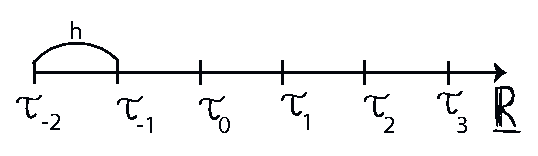
\includegraphics{35.eps}\\
\
На сетке $B$ из предыдущего пункта локальный B-сплайн(базисный) 3-ей степени $S^{(i)}$ имеет вид	
\begin{gather*}
	S^i(\tau) = 
	\begin{cases}
		x^3, \;\; x = \frac{\tau - \tau_{i-2}}{\tau_{i-1} - \tau_{i-2}}, \;\; \tau \in [\tau_{i-2}, \tau_{i-1}]\\
		1 + 3x + 3x^2 - 3x^3, \;\; x = \frac{\tau - \tau_{i-1}}{\tau_i - \tau_{i-1}}, \;\; \tau \in [\tau_{i-1}, \tau_i]\\
		4 - 6x^2 + 3x^3, \;\; x = \frac{\tau - \tau_{i+1}}{\tau_{i+1} - \tau_{i}}\\
		(1-x)^3, \;\; x = \frac{\tau_i - \tau_{i+2}}{\tau_{i+2} - \tau_{i+1}}, \;\; \tau \in [\tau_{i+1}, \tau_{i+2}]\\
		0, \;\; \tau \notin [\tau_{i-2}, \tau_{i+2}]
	\end{cases}
\end{gather*}
Построение пространству $Spl_2(A)$ строится пространство $Spl_3(A)$ B-сплайнов 3-ей степени с базисом:
\begin{gather*}
	H = \langle h_0, h_1, ..., h_k \rangle,
\end{gather*}
где $h_i = S^{(i)}|_{[a, b]}$ для $i = \overline{0,k}$\\
Тогда интерполируемый локальный $B$-сплайн на сетке $A = \langle \tau_0, \tau_1, ..., \tau_k \rangle S^{(3)}(A, \;^>y)$ для $A$-сеточной функции $^>y = [ y_0, y_1, ..., y_k \rangle \in\; ^> \mathbb{R}^{|A|}(A)$ имеет вид 
\begin{gather}
S^{(3)}(A, \;^>y) = \sum_{i=0}^{k}{z_iS^{(3)}(A, \;^>e_{i+1})},
\label{36-S3}	
\end{gather}
где $S^{(3)}(A, \;^>e_{i+1}) = h_i$ для $i = \overline{0,k}$\\
Вектор $^>z = [ z_0, z_1, ..., z_k \rangle$ для вида \ref{36-S3} определяется из СЛАУ
\begin{gather*}
	\begin{pmatrix}
		4 & 1 & 0 & . & . & . & 0\\
		1 & 4 & 1 & 0 & . & . & 0\\
		0 & . & . & . & . & . & 0\\
		. & . & . & . & . & . & .\\
		. & . & . & . & . & . & .\\
		. & . & . & . & . & . & .\\
		0 & . & . & 0 & 0 & 1 & 4\\				
	\end{pmatrix}
	\;^>z = \;^>y \leftrightarrow C\;^>z = \;^>y
\end{gather*}
Поскольку $C$ имеет диагональное преобладание 2, то $\exists C^{-1}$ и $||C^{-1}||\leq \frac{1}{2}$
\end{document}